\section{System design}
\begin{figure}[t]
	\centering
	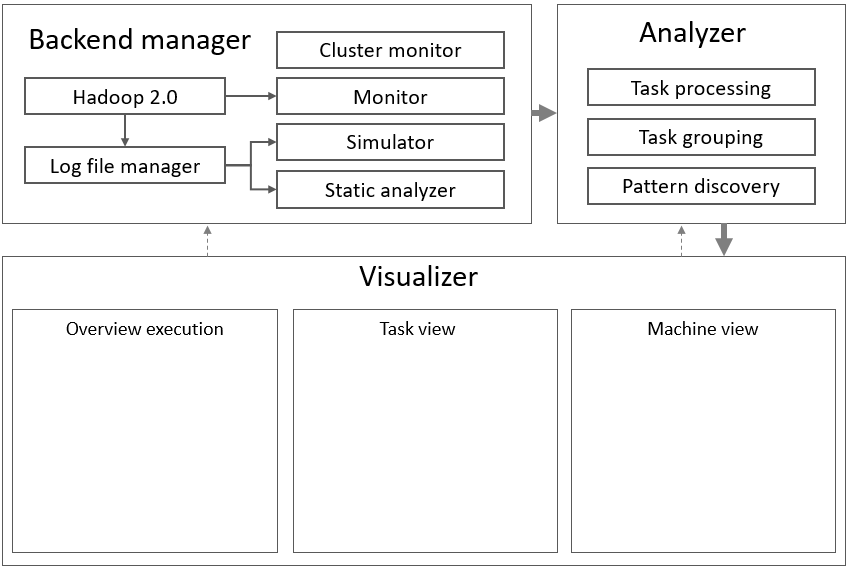
\includegraphics[width=0.49\textwidth]{figures/system/sysdesign.png}
	\vspace{-3mm}
	\caption{$\DQV$ system consists of three major components: backend manager, analyzer and visualizer.}
	\label{fig:sysdesign}
	\vspace{-3mm}
\end{figure}
As shown by Figure~\ref{fig:sysdesign}, $\DQV$ consists of three modules: backend manager, analyzer, and visualizer. 

In our current system, we use Hadoop2.0 as the\textbf{ distributed query engine}. The system can run in three modes: monitoring mode, simulation mode and analytics mode. The monitoring mode directly collect the real-time execution log from Hadoop2.0, then process it and send the result to analyzer. The simulator and log analyzer are linked with log file manager, a module to process and save logs as as structured data form. Log analyzer directly output the strusctured data to the next module. The simulator simulatses the execution progress which allow users to adjust the running speed and explore the dynamic query process. 

The analyzer collects the data from the backend manager and further process them for visualization. 

The visualization module integrates coordinated views to support interactive exploration of and reasoning about the query behaviour at the different perspectives. Execution overview demostrates the execution process in at the vertex level. A new algorithm for the temporal DAG is proposed to visualize the structure and process at the same time. The task view visualize the temporal information of tasks as well as the dataflow relationship among the tasks. The profiling view integrates the task view with the resource status for each machines.  A rich set of interactions are also supported to link different views together.


